\hypertarget{program-verification}{%
\section{Program Verification}\label{program-verification}}

\begin{itemize}
\tightlist
\item
  What are the basic ideas of verification?

  \begin{itemize}
  \tightlist
  \item
    the problem of erroneous software; correctness; knowing correctness;
    specification and implementation
  \end{itemize}
\item
  Basic theory of verifying imperative programs
\item
  An in principle understanding of verification technology
\item
  at the end, students should be in a good starting position for using
  actual verification tools like Dafny
\item
  besides that, knowing these points increases one's repertoire of
  possibilities to think about software
\end{itemize}

\hypertarget{software-qualities}{%
\subsection{Software Qualities}\label{software-qualities}}

\begin{itemize}
\tightlist
\item
  Reliability: correctness, robustness

  \begin{itemize}
  \tightlist
  \item
    efficiency, usability etc. irrelevant as long as software is not
    reliable
  \end{itemize}
\item
  Dependability: knowing that software is reliable

  \begin{itemize}
  \tightlist
  \item
    reliability itself is not enough --- we must know that software is
    reliable
  \end{itemize}
\end{itemize}

\hypertarget{iml}{%
\subsection{IML}\label{iml}}

\begin{itemize}
\tightlist
\item
  IML is a simple imperative programming language augmented with
  specification constructs
\item
  under development for this course to demonstrate the basic principles
  of program verification
\item
  its only data types are integers and booleans
\item
  IML: Imperative Mini Language
\end{itemize}

\begin{lstlisting}
specification
requires a >= 0
modifies r
ensures r*r <= a && a < (r+1)*(r+1)
\end{lstlisting}

\begin{itemize}
\tightlist
\item
  the requires clause declares a precondition
\item
  the modifies clause declares a framecondition

  \begin{itemize}
  \tightlist
  \item
    this is a list of variables that are allowed to be changed, but the
    central idea is that all other variables remain constant
  \end{itemize}
\item
  the ensures clause declares a postcondition
\end{itemize}

This IML statements declare actually followin code:

\begin{lstlisting}
int f(int a)
{
    int t, s, i;
    t= 1; s= 1; i= 0;
    while (s <= a) {
        t= t + 2;
        s= s + t;
        i= i + 1;
    }
    return i;
}
\end{lstlisting}

\hypertarget{example}{%
\subsubsection{Example}\label{example}}

We skipped somehow the most of the grammar in IML, but we took a look in
the following example (not in detail).

\begin{lstlisting}
specification
    requires a > 0 && b > 0
    modifies x
    ensures x = gcd(a, b)
implementation
    x := a;
    y := b;
    while x != y
        invar gcd(x, y) = gcd(a, b) && x > 0 && y > 0
    do
        if x > y then
            x := x - y
        else
            y := y - x
        end
    end
\end{lstlisting}

\begin{itemize}
\tightlist
\item
  gcd(a, b) denotes the greatest common divisor of a and b
\item
  we use gcd in the postcondition to specify that our program computes a
  gcd
\item
  we use gcd in the while loop (after invar) for verification purposes
\item
  the meaning of invar in the while loop will be carefully discussed
  later
\item
  Note: the red phrases are assertions; those containing gcd could not
  occur as boolean expressions in if or while (see grammar!)
\end{itemize}

\clearpage
\hypertarget{specification-vs.implementation}{%
\subsubsection{Specification
vs.~Implementation}\label{specification-vs.implementation}}

\begin{itemize}
\tightlist
\item
  the specification describes what the function does without explaining
  how to do it
\item
  the implementation describes how to compute the function without
  explaining what the result will be
\end{itemize}

When we need both specification and implementation, then simply let us
put both of them together to form the program.

Specification AND implementation in Dafny:

\begin{lstlisting}
method NatSquareRootA(a:int) returns (r:int)
    requires a >= 0;
    ensures r*r <= a < (r+1)*(r+1);
{
    var d:int;
    var s:int;
    d := 1; // oDd
    s := 1; // Square
    r := 0; // Root
    while (s <= a)
        invariant d == 2*r + 1;
        invariant s == (r+1)*(r+1);
        invariant r*r <= a;
    {
        d := d + 2;
        s := s + d;
        r := r + 1;
    }
}
\end{lstlisting}

\hypertarget{dafny}{%
\subsection{Dafny}\label{dafny}}

Dafny is a specification and implementation language to proving the
correctness of an implementation against a specification.

Since very special knowledge is needed for developing an implementation
from a specification, it is not reasonable to assume that it could be
possible to construct a compiler that compiles a specification into
executable code.

\hypertarget{validation-vs-verification}{%
\subsection{Validation vs
Verification}\label{validation-vs-verification}}

\textbf{Validation}: Does the specification fulfill the requirements?\\
\textbf{Verification}: Does the implementation fulfill the
specification?

\begin{figure}[H]
\centering
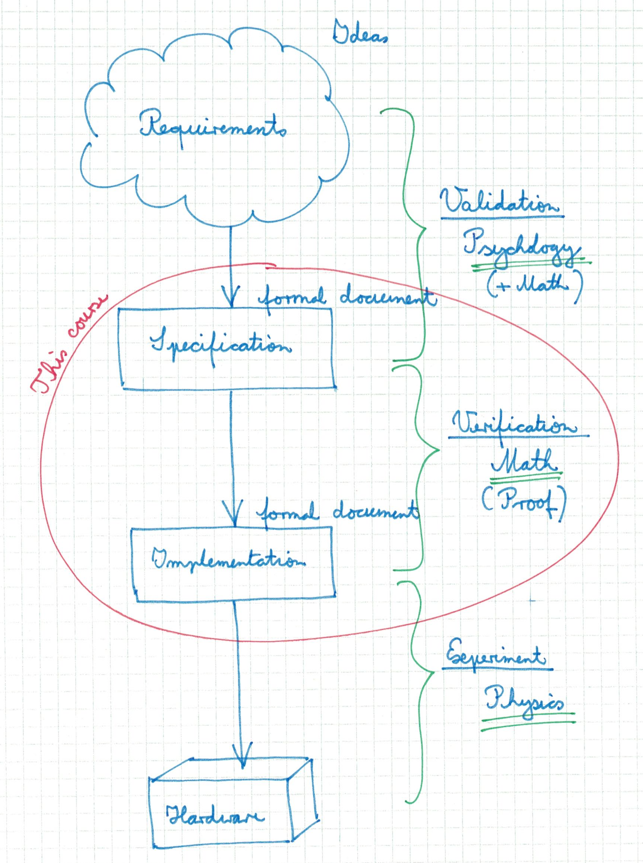
\includegraphics[width=0.5\textwidth]{figures/validationverification.png}
\caption{Validation and Verification}
\end{figure}

Focus on verification:

\begin{itemize}
\tightlist
\item
  Specification and implementation

  \begin{itemize}
  \tightlist
  \item
    two descriptions of the same problem, and that with different points
    of view
  \item
    redundancy
  \end{itemize}
\item
  How to Know Consistency?

  \begin{itemize}
  \tightlist
  \item
    Testing
  \item
    Proving
  \item
    Combination of both
  \end{itemize}
\end{itemize}

\hypertarget{testing}{%
\subsubsection{Testing}\label{testing}}

\begin{itemize}
\tightlist
\item
  program will be executed on chosen input
\item
  is output consistent with specification?

  \begin{itemize}
  \tightlist
  \item
    yes: no (nearly no) knowledge gained
  \item
    no: now we know more: that the program contains an error
  \end{itemize}
\end{itemize}

\begin{tcolorbox}[colback=red!5!white,colframe=red!75!black]
\textbf{Dijkstra's famous statement} \\
"The number of different inputs, i.e. the number of different computations for which the assertions claim to hold is so fantastically high that demonstration of correctness by sampling is completely out of the question. Program testing can be used to show the presence of bugs, but never to show their absence!"
\end{tcolorbox}

In other words: A successful industrial acceptance test does not mean
that a software product is free of errors; it just means that the
customer has to pay

\hypertarget{proving}{%
\subsubsection{Proving}\label{proving}}

\begin{itemize}
\tightlist
\item
  program will not be executed
\item
  rather we try to find a mathematical proof
\item
  do we find a proof?

  \begin{itemize}
  \tightlist
  \item
    yes: now we know that the program is correct
  \item
    no: we know that the program might contain errors, or a good idea
    for the proof is (still) missing
  \end{itemize}
\end{itemize}

\hypertarget{testing-and-proving}{%
\subsubsection{Testing and Proving}\label{testing-and-proving}}

\begin{itemize}
\tightlist
\item
  Testing: good for finding bugs
\item
  Proving: good for showing that there are no bugs
\item
  good practical method:

  \begin{itemize}
  \tightlist
  \item
    first: test your program to find as many errors as possible
  \item
    then: try to prove your program correct
  \end{itemize}
\end{itemize}

\clearpage
\hypertarget{state}{%
\subsection{State}\label{state}}

\begin{itemize}
\tightlist
\item
  the distinguishing feature of any imperative programming language is
  the explicit manipulation of state
\item
  the state of an imperative program can be modelled as a function that
  maps the variables (VAR) of a program to their current contents (VAL):

  \begin{itemize}
  \tightlist
  \item
    STATES = VAR -\textgreater{} VAL
  \item
    $\sigma$1, $\sigma$2, $\sigma$3, $\sigma$4 : STATES
  \end{itemize}
\end{itemize}

\begin{lstlisting}
$\sigma$1(x) = 17, $\sigma$1(y) = 5
x := x - y;
$\sigma$2(x) = 17 - 5 = 12, $\sigma$2(y) = 5
y := x + y;
$\sigma$3(x) = 12, $\sigma$3(y) = 12 + 5 = 17
x := y - x
$\sigma$4(x) = 17 - 12 = 5, $\sigma$4(y) = 17
\end{lstlisting}

\hypertarget{boolean-expressions}{%
\subsection{Boolean Expressions}\label{boolean-expressions}}

\begin{itemize}
\tightlist
\item
  given a boolean expression and a state

  \begin{itemize}
  \tightlist
  \item
    boolean expression either true or false
  \end{itemize}
\item
  condition in if or while command

  \begin{itemize}
  \tightlist
  \item
    condition will be evaluated; yields either true or false
  \end{itemize}
\item
  condition as assert command

  \begin{itemize}
  \tightlist
  \item
    should always yield true; if it does not, the program is in error
  \end{itemize}
\end{itemize}

\hypertarget{assertions}{%
\subsection{Assertions}\label{assertions}}

\begin{itemize}
\tightlist
\item
  in programming languages like Java, the assert commands contain
  boolean expressions that can be evaluated at run time
\item
  in verification languages like IML or Dafny, the assert commands
  contain assertions
\item
  an assertion describes a set of states: the set of all states that
  satisfy the assertion

  \begin{itemize}
  \tightlist
  \item
    the assertion `x \textgreater{} 5' describes the set of all states
    with $\sigma$(x) \textgreater{} 5, for example
  \item
    $\sigma$1 with $\sigma$1(x) = 6 and $\sigma$1(y) = 25, or
  \item
    $\sigma$2 with $\sigma$2(x) = 17 and $\sigma$2(y) = 35
  \item
    the assertion `true' describes the set of all states that satisfy
    true, that is, the full set of all possible states
  \end{itemize}
\end{itemize}

\hypertarget{implication}{%
\subsection{Implication}\label{implication}}

\begin{figure}[H]
\centering
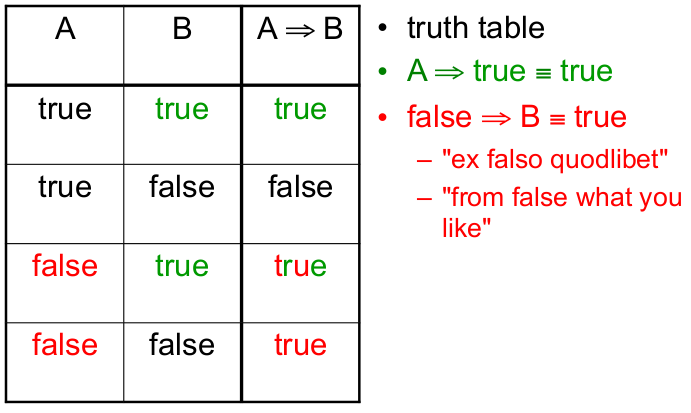
\includegraphics[width=0.5\textwidth]{figures/implication.png}
\caption{Implication}
\end{figure}

\begin{itemize}
\tightlist
\item
  ``If I win, I'll eat my hat.''
\item
  is true

  \begin{itemize}
  \tightlist
  \item
    if I do not win (independent of what I will do with my hat) --- ex
    falso quodlibet
  \item
    if I win and I eat my hat
  \end{itemize}
\item
  is false

  \begin{itemize}
  \tightlist
  \item
    if I win but I do not eat my hat
  \end{itemize}
\end{itemize}

\begin{figure}[H]
\centering
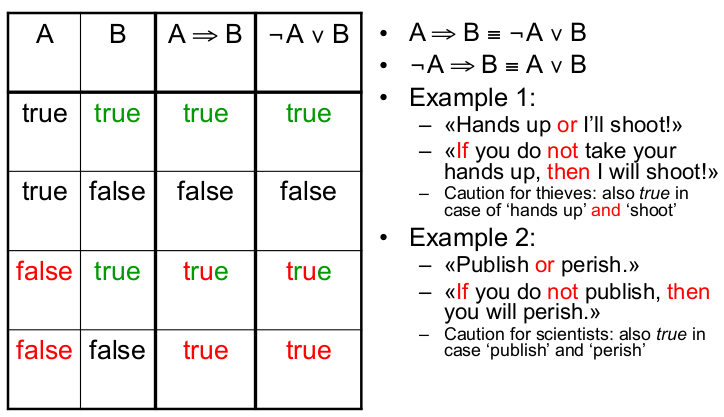
\includegraphics[width=0.7\textwidth]{figures/implication2.png}
\caption{Implication 2}
\end{figure}

\begin{itemize}
\tightlist
\item
  implication has nothing to do with causal relations; just the truth
  table matters
\item
  if A is false, the implication will always be true.
\end{itemize}

\clearpage
\hypertarget{weaker-and-stronger-conditions}{%
\subsubsection{Weaker and Stronger
Conditions}\label{weaker-and-stronger-conditions}}

\begin{itemize}
\tightlist
\item
  examples:

  \begin{itemize}
  \tightlist
  \item
    x = 5 $\land$ y = 7 -\textgreater{} x = 5
  \item
    x = 5 -\textgreater{} x = 5 $\lor$ y = 7
  \end{itemize}
\item
  P -\textgreater{} Q

  \begin{itemize}
  \tightlist
  \item
    P more restrictive than Q
  \item
    set of states given by P is subset of set of states given by Q
  \item
    P stronger than Q
  \item
    Q weaker than P
  \end{itemize}
\item
  boundary cases:

  \begin{itemize}
  \tightlist
  \item
    What is the strongest condition? --\textgreater{} False
  \item
    What is the weakest condition? --\textgreater{} True
  \end{itemize}
\end{itemize}

\hypertarget{validity-versus-truth}{%
\subsubsection{Validity Versus Truth}\label{validity-versus-truth}}

\begin{itemize}
\tightlist
\item
  A boolean formula B (for example an assertion or a Hoare triple) is
  valid if it is true in all states, written $\models$ B.

  \begin{itemize}
  \tightlist
  \item
    x + 5 = 5 + x is true in all states
  \item
    thus x + 5 = 5 + x is valid: $\models$ x + 5 = 5 + x
  \end{itemize}
\end{itemize}

\clearpage
\hypertarget{hoare-triples}{%
\subsection{Hoare Triples}\label{hoare-triples}}

A Hoare triple consists of

\begin{itemize}
\tightlist
\item
  an assertion P, called the \textbf{precondition} of the Hoare triple
\item
  a command C
\item
  an assertion Q, called the \textbf{postcondition} of the Hoare triple
\end{itemize}

\textit{Note: P and Q are the precondition and postcondition of the Hoare
triple, not precondition and postcondition of the command}

\begin{lstlisting}
{ x = 5 } x := x + 1 { x = 17 }
{ x > 5 } x := x + 1 { x > 6 }
{ j = 0 } while i = 0 do skip endwhile { k = 0 }
\end{lstlisting}

\begin{itemize}
\tightlist
\item
  a Hoare triple itself is a boolean formula, which can be true in some
  state and false in others
\item
  we call the state in which execution of C begins the \textbf{prestate}
  of that execution, and the resulting state its \textbf{poststate}, the
  latter provided that execution terminates
\end{itemize}

\begin{tcolorbox}[colback=red!5!white,colframe=red!75!black]
((prestate satisfies P $\wedge$ execution of C terminates) $\Rightarrow$ poststate satisfies Q)
\end{tcolorbox}

\begin{itemize}
\tightlist
\item
  This means, if the prestate is wrong, the full Hoare tripple is true
  (since it's an implication)
\item
  The prestate also includes the termination of the program c. If the
  program doesn't terminate, everything is ok
\end{itemize}

\begin{figure}[H]
\centering
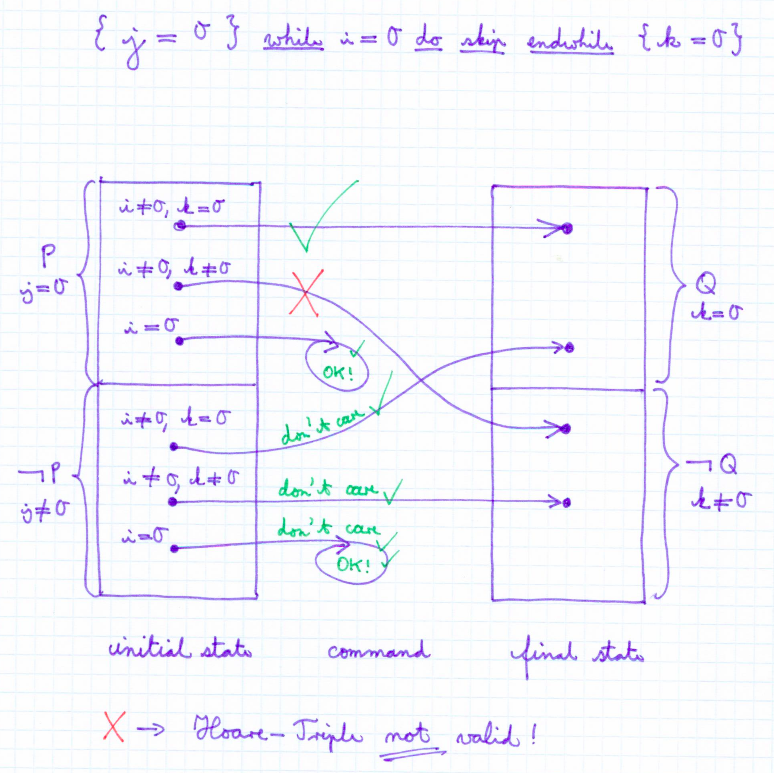
\includegraphics[width=0.6\textwidth]{figures/hoaretriple.png}
\caption{Hoare Triple example}
\end{figure}

\begin{itemize}
\tightlist
\item
  given the following Hoare triple:

  \begin{itemize}
  \tightlist
  \item
    \{ j = 0 \} while i = 0 do skip endwhile \{ k = 0 \}
  \end{itemize}
\item
  The example above describes all 8 kinds of prestates (i = 0 implies 2
  states each).
\item
  The example shows, that the hoare triple would be false in one
  prestate and thus the hoarse triple itself is not valid.
\end{itemize}

\hypertarget{conditional-or-partial-correctness}{%
\subsubsection{Conditional or Partial
Correctness}\label{conditional-or-partial-correctness}}

\begin{itemize}
\tightlist
\item
  A Hoare triple \{P\} C \{Q\} is called \textbf{valid}, written $\models$ \{P\}
  C \{Q\} if it is true in all prestates.
\item
  A Hoare triple is valid, If execution of command C begins in any state
  that satisfies the precondition P and execution terminates, then the
  resulting state satisfies the postcondition Q.
\item
  Note that a valid Hoare triple does not provide any information
  concerning the resulting state if execution begins in any state that
  does not satisfy the precondition.
\item
  We are only interested in valid Hoare triples.
\end{itemize}

\begin{tcolorbox}[colback=red!5!white,colframe=red!75!black]
Examples: \\
– $\nvDash$ { x = 5 } x := x + 1 { x = 17 } (this is not valid, since the postcondition could not be met) \\
– $\models$ { x > 5 } x := x + 1 { x > 6 } \\
– $\nvDash$ { j = 0 } while i = 0 do skip endwhile { k = 0 }
\end{tcolorbox}

\hypertarget{total-vs.partial-correctness}{%
\subsubsection{Total vs.~Partial
Correctness}\label{total-vs.partial-correctness}}

\begin{itemize}
\tightlist
\item
  If the precondition is true, the execution terminates properly and the
  postcondition is true, the Hoare triple is called totally correct.
\item
  If you don't know if the execution terminates properly, but if it
  terminates the result is true, the Hoare triple is called partially
  correct.
\end{itemize}

\hypertarget{specification-of-imperative-programs}{%
\subsection{Specification of Imperative
Programs}\label{specification-of-imperative-programs}}

A specification for imperative programs should provide the following
information:

\begin{itemize}
\tightlist
\item
  a precondition P
\item
  a list x of variables that may be changed

  \begin{itemize}
  \tightlist
  \item
    with the important understanding that all other variables must not
    be changed
  \end{itemize}
\item
  a postcondition Q
\end{itemize}

We denote such a specification by \{P\} x:=? \{Q\}

\hypertarget{specification-for-integer-square-root}{%
\subsubsection{Specification for Integer Square
Root}\label{specification-for-integer-square-root}}

\begin{itemize}
\tightlist
\item
  English spec

  \begin{itemize}
  \tightlist
  \item
    Find an integer approximation to the square root of integer a.
  \end{itemize}
\item
  add precision

  \begin{itemize}
  \tightlist
  \item
    a $\geqslant$ 0
  \item
    store result in variable r
  \item
    choose largest integer r such that $r^2$ $\leqslant$ a
  \end{itemize}
\item
  formal spec

  \begin{itemize}
  \tightlist
  \item $\{0 \leqslant a\} r:=? \{r^2 \leqslant a < (r + 1)^2\}$
  \end{itemize}
\end{itemize}

It is important to list all the variables that are allowed to be changed
(r := ?). If we would not define that, we could change a to 0 to meet
the conditions.

\hypertarget{rigid-variables}{%
\subsubsection{Rigid Variables}\label{rigid-variables}}

Rigid variables can be introduced to connect the pre- and the
postconditions with variables that only occur in assertions and not in
the program.

\{ x = X \} x:=? \{ x = X + 6 \}

this means: for all values X, if x = X in the initial state and
execution terminates, then x = X + 6 in the final state.

\clearpage